%%%%%%%%%%%%%%% Updated by MR March 2007 %%%%%%%%%%%%%%%%
\documentclass[12pt]{article}
\usepackage{a4wide}
\usepackage{graphics}       % Graphics commands



\newcommand{\al}{$<$}
\newcommand{\ar}{$>$}

\parindent 0pt
\parskip 6pt

\begin{document}

\thispagestyle{empty}

\rightline{\large{Ciaran Deasy}}
\medskip
\rightline{\large{Churchill College}}
\medskip
\rightline{\large{cfd27}}

\vfil

\centerline{\large Computer Science Tripos, Part II}
\vspace{0.4in}
\centerline{\Large\bf A Prolog Compiler with Continuations}
\vspace{0.3in}
\centerline{\large 2013/14}
\vspace{2.5in}

\newpage
\hspace{5px}
\newpage

\vfil

\centerline{\large Ciaran Deasy, Churchill College}
\vspace{0.4in}
\centerline{\Large\bf A Prolog Compiler with Continuations}
\vspace{0.3in}
\centerline{\large Computer Science Tripos, Part II, 2014}
\vspace{0.1in}
\centerline{ ***** words}
\vspace{0.25in}

{\bf Author:} Ciaran Deasy\\
{\bf College:} Churchill College

\vspace{0.25in}

{\bf Project Originator:} Alan Mycroft\\
{\bf Project Supervisor:} Alan Mycroft

\vspace{0.25in}

{\bf Aim:}\\
The purpose of this project was to produce two implementations of the Prolog programming language, one being an interpreter and the other a compiler outputting source ML code. 
The implementations were to be written in ML and use continuation-passing style to implement the traditionally awkward backtracking behaviour of Prolog in a simple and intuitive way. 
The implementations were to be extensive, covering the important features of Prolog and capable of running many useful programs, but not a complete or exhaustive realisation.

\vspace{0.25in}

{\bf Work completed:}\\
Both implementations of Prolog were completed as planned. 
They were tested for correctness on a wide range of sample programs, and their relative performance was measured. 
Continuation-passing style was successfully leveraged in the implementations.

\vspace{0.25in}

{\bf Special Difficulties:} None

{\bf Declaration of Originality:}
I, Ciaran Deasy of Churchill College, being a candidate for Part II of the Computer Science Tripos, hereby declare that this dissertation and the work described in it are my own work, unaided except as may be specified below, and that the dissertation does not contain material that has already been used to any substantial extent for a comparable purpose. 

Signed %TODO

Date %TODO

\vfil
\eject

\tableofcontents 

\newpage

\section{Introduction}

% Introduction and Preparation: 3100 words

\subsection{Project Overview}

The purpose of this project was to produce two implementations of the Prolog programming language, written in ML. 
The first implementation was an interpreter.
It would take as input a source file containing Prolog program clauses and queries, and for each query, run it against the program clauses. 
It would output whether the query succeeded, and if it did, the bindings assigned to query variables.
The second implementation was a compiler, taking the same input. 
This would output an ML source file which, when itself compiled and run, would give the same output as the interpreter.
The internal implementation was to use continuation-passing style, a technique that has been previously used to good effect to implement backtracking algorithms, with the aim of deciding whether this was a useful and intuitive way of implementing the Prolog language. 
The project also sought to investigate the potential performance gains of pre-compiling a Prolog program, compared with simply interpreting it.

\subsection{Prolog}

Prolog is a declarative programming language. 
Unlike imperative languages like Java, or functional languages like ML, programs written in Prolog do not define algorithms by specifying a sequential list of operations. 
Instead, constraints are placed on variables, and it is left to the Prolog implementation to determine variable bindings that satisfy those constraints. 

\subsubsection{Terms}

Prolog's only datatype is the term. 
A term can be either an atom, a variable or a compound term. 
An atom is a numerical or string literal. 
A variable is an unbound term which can be bound to any other term, such that that term replaces all occurrences of the variable. 
A compound term consists of a functor symbol, which is just a string literal, and one or more argument terms.

Prolog also supports lists of terms of the recursive form \verb/[H|T]/, where \verb|H| is the first term of the list and \verb|T| is another list containing all of the other terms.

\subsubsection{Clauses}

Prolog programs are made up of clauses. 
A clause consists of a head term and a list of body terms, with the semantic meaning that the head term is true if the body terms can be shown to be true. 
Syntactically, it is written as \verb|Head :- Body|$_1$\verb|, ..., Body|$_n$\verb|.|

Prolog clauses are based on Horn clauses in first-order logic. 
A Horn clause is a disjunction of literals containing at most one positive literal. 
The body terms in a Prolog clause correspond to the negated literals in a Horn clause, and the head term corresponds to the positive literal. 
If all of the body terms can be shown to be true, then for the Horn clause to be true, it must be the case that the head term is true. 

A set of clauses whose head terms have the same functor symbol and arity (number of argument terms) constitute a predicate, and the functor symbol and arity are analogous to a function signature: a fact that this project will exploit when compiling to source ML.

A clause with no body terms is often called a fact, because as a disjunction of one positive literal, it simply asserts that something is always true.

\subsubsection{Queries}

A Prolog query contains a list of query terms. 
The goal of a Prolog implementation is to exhibit a set of consistent bindings on variables in the query such that the program clauses prove every term in the query to be true, or to establish that no such set of bindings exists. 
Syntactically, it is written as \verb|:- QueryTerm|$_1$\verb|, ..., QueryTerm|$_n$\verb|.|

\subsubsection{Unification}

The most important operation in Prolog is unification of terms. 
Two instantiated atoms unify if they are equal. 
A variable can be made to unify with any other term by binding it to that term. 
Two compound terms unify if they have the same functor symbol and the same arity, and each $i$th argument in one term unifies with the corresponding $i$th argument in the other term. 
Performing unification in Prolog involves finding a consistent set of variable bindings such that two input terms unify successfully, or determining that no such set exists. 
A set of variable bindings is consistent if no variable is bound to two distinct and non-unifiable terms. 
For a successful unification, the variable bindings must be consistent not only with each other, but with all variable bindings made by earlier unifications.

\subsubsection{Control Flow and Backtracking}

A Prolog term is successfully executed if it unifies with the head of a clause, and each term in the body of the clause is successfully executed.
Prolog execution proceeds by successively executing each term in a query. 
If all query terms are executed successfully, then the variable bindings that had to be made are returned.

When executing a term, a clause is selected with which to try to unify it.
If at any point in Prolog execution a unification fails, then control backtracks to the last time a clause selection was made, and selects a different clause.
Any variable bindings that were made since that selection are undone.
If there are no more clauses to try, then control backtracks further, to the selection before that.
If there is no point to backtrack to, then query execution is said to have failed.

\subsubsection{Cut}

Prolog's cut operator, written `\verb|!|', is a special term which clears certain existing backtracking points.
When it is reached during execution of the body terms in a clause, we are no longer allowed to backtrack to the execution of body terms that appear before it in the clause. 
We are also no longer allowed to try another clause for the current execution of the current term. 
Failure must backtrack to an earlier term's execution.

\subsubsection{Occurs Check}

A Prolog variable is said to trigger the occurs check if it is bound to a term containing itself.
For example, if we had a binding \verb|A = a(A)|, this would trigger the occurs check.
Typical Prolog implementations will accept such a binding, and mine are no exception.
However, it should be clear that some care will likely be needed when substituting variables to handle bindings like these in a clean way.
When I discuss substitutions in \S3.9, I will talk briefly about this.

\subsubsection{Arithmetic Evaluation}

Prolog implementations support the same standard arithmetic expressions that most other languages do.
An expression \verb|1+2*6-4| can be written and is accepted as Prolog syntax.
However, what may be surprising is that this doesn't implicitly get evaluated down to \verb|9|. 
Rather, this syntax is shorthand for the Prolog term \verb|-(+(1,*(2,6)),4)|.
Indeed, if we were to try to unify this with the term \verb|9|, it would fail.
The special two-argument in-fix predicate `\verb|is|' is provided by Prolog implementations to perform arithmetic evaluation.
The second argument provided to \verb|is| will be evaluated as one would expect for arithmetic, and then unified with the first argument.
So \verb|9 = +(6,3)| would fail, but \verb|9 is +(6,3)| would succeed.

\subsection{The Byrd Box Model}

A helpful description of Prolog's control flow is given by the Byrd box model. 
A typical programming function can be modelled as a box with two ports: a ``call'' port for calling into the function and a ``success'' port when the function returns. 
Once a function call returns, it is never re-entered.
In Prolog, however, a predicate may find zero, one, or many answers to a call. 
If there is no solution, then control leaves through a ``fail'' port, and enters an earlier predicate's ``redo'' port.
A Prolog predicate is therefore viewed as a procedure with four ports: two ways in which control can be passed to the predicate, and two ways in which it can leave.
This is called the Byrd box model.
A deeper specification of this model is given by Jahier et al. \cite{byrd00}

\subsection{The WAM}

Warren's Abstract Machine (``the WAM'') is the most common basis for implementing Prolog. 
It consists of a memory architecture and an instruction set. 
The memory architecture describes a systematic way to efficiently lay out Prolog terms in a heap structure, while the instruction set describes operations for manipulating this structure, corresponding to familiar primitive Prolog operations like unification. 

Clearly from the above description of the Byrd box model, it is necessary to have some mechanism that maintains information about predicate evaluations so that they can be re-entered through the ``redo'' port. 
To this end, the WAM also describes a stack of environments, whereby the bindings made by unifying terms when evaluating predicates are tracked so that they can be undone in the event of backtracking. 

A full discussion of the WAM's design is given by A\"it-Kaci \cite{wam91}.

This project does not follow the WAM's model. 
Rather, the focus is on leveraging ML's language features to achieve a cleaner, simpler and more intuitive implementation of Prolog. 
In particular, I will describe in \S2.1 how the use of continuation-passing style removes the need for the WAM's environment stack by using ML's function closures to implicitly retain the required information.

\newpage

\section{Preparation}

% Introduction and Preparation: 3100 words

\subsection{Pure Prolog}

The success criterion for the project is succinctly described as an implementation of ``pure'' Prolog. 
However, pure Prolog is not an entirely well-defined delineation, so before commencing work on the project, I needed to expressly define pure Prolog to clarify the goals of the implementations.

Pure Prolog includes Horn clauses of the syntactic form \verb|Head :- Body.|, where \verb|Head| is a positive literal \verb|h| and \verb|Body| is a comma-separated list of positive literals \verb|b_1, ..., b_n| $(\verb|n| > 0)$. 
It also includes query terms of the syntactic form \verb|:- q_1, ..., q_n.| $(\verb|n| > 0)$.

Pure Prolog does not include any built-in predicates, such as \verb|atomic/1|. 
It also excludes arithmetic infix operators like \verb|+| and \verb|-|, and the \verb|is| keyword. 
It does not include the cut operator \verb|!|.

The final project was extended to include several of these elements, including arithmetic evaluation, the cut operator, and a selection of built-in predicates.
However, the implementations are not an exhaustive realisation of the full standard Prolog language, nor were they intended to be.

\subsection{Programming in Continuation-Passing Style}

Typically in programming, we work with functions or procedures of some kind. 
A function call takes some parameters, branches to another point of code, computes a result, and branches back to the point of calling to continue execution.

Continuation-Passing Style (CPS) is an alternative to this paradigm. 
In pure CPS, there is no concept of ``returning'' a value. 
When a function $f$ is called, it is provided with a continuation $k$ as one of its parameter, which is a function representing the next step of computation after $f$ completes. 
If $f$ computes values which need to be passed on, the $k$ can specify appropriate parameters to facilitate this.

The usefulness of CPS becomes clear when one considers giving multiple continuation functions, say $k1$ and $k2$, to a function $f$. 
This gives an elegant way of forking execution in two or more directions. 
In a non-CPS program, such a fork would require $f$ to return a value and then its caller would test the value and choose a direction of execution on that basis. 
In CPS, $f$ doesn't have to encode the information in a type-restricted return value.

The software produced for this project uses a mixture of conventional style and CPS. 
The unification algorithm is implemented in conventional style: it accepts two terms to unify and a set of the existing variable bindings that must remain consistent, and returns the updated set of substitutions. 
CPS is leveraged in the interpreter and in compiled output to implement the backtracking control flow of Prolog.
The way in which this is done maps directly onto the Byrd box model described in \S1.3. When we enter a predicate for the first time through the ``call'' port, we are given a success continuation corresponding to the ``success'' port and a failure continuation corresponding to the ``fail'' port and leading to a previous predicate's ``redo'' port.

\subsection{ML as an implementation language}

I studied ML as part of the first year course, but it was in the context of an introduction to the foundations of Computer Science. 
Thus, the actual ML proficiency that was taught did not go beyond a very basic level, with programs consisting of just a couple of functions which were a handful of lines long. 
There is a large gap between a simple sorting algorithm and an implementation of a programming language. 
To address this, I spent a portion of my preparation time studying ``ML for the Working Programmer'', a standard textbook on the language, to develop the necessary proficiency and learn the use of advanced ML concepts like modules that help with programming at the necessary scale.

The was no strong motivation to favour any particular variant of ML over another.
I chose Standard ML of New Jersey (SML/NJ) because of an informal impression that it was the most frequently referenced variant in the literature I encountered.

\newpage

\section{Implementation}

% Implementation: 4700 words

\subsection{Unit Testing}

Being a relatively little-used language, particularly for building substantial pieces of software, the libraries available for ML are quite limited. 
With regard to unit testing, the main library I came across was SMLUnit. 
I looked into using it, but found that while it would work, it was a very heavyweight solution.

The alternative approach was to write my own unit testing framework. 
I looked into this, and found that it could be done very easily. 
ML is not completely free of side-effects, but code written in ML tends towards having very few, which makes it very amenable to simple unit testing. 
Thus, I was able to write a very small unit tester - about 40 lines of code - that was sufficient for the needs of this project.

The main function is \verb|checkResult()|, which takes a test name, the actual and expected results of a function, and a function for comparing the two. 
It prints success or failure as appropriate. 
It maintains two internal counters for the number of tests which pass or fail, and a \verb|conclude()| function to be called at the end of a test run to print and reset the counters.

A set of test cases is simply a function consisting of calls to \verb|checkResult()|, and ending with a call to \verb|conclude()|.

It was important, of course, that the unit tester be completely correct so that test failures would be properly detected. 
To ensure this, I had the code for the unit tester code-reviewed by a fellow Part II student.

\subsection{Datatypes}

For the implementations, a hierarchy of datatypes were needed to represent Prolog programs, as well as datatypes to represent the interpreter's and compiler's internal state. The details of these datatypes are discussed below.

\subsubsection{Lexer tokens}

A \verb|token| datatype was needed to represent the token types that could be recognised during lexing, as will be described in \S3.4. 
The \verb|INT|, \verb|FLOAT|, \verb|ATOM| and \verb|VARIABLE| tokens appear as ML constructors and contain relevant values, while all other token types have no internal values. 
The only noteworthy aspect of this datatype is that, because the \verb|FLOAT| token needs to contain a value of type \verb|real| which isn't an equality type in ML, the \verb|token| datatype isn't an equality type. 
Thus, an explicit equality function had to be defined.

\subsubsection{Terms}

At the bottom level, we have four types of \verb|term|s. 
A \verb|Term|\footnotemark[1] is a typical instantiated Prolog term, consisting of a \verb|Functor| string and a list of \verb|term|s representing its arguments. 
An atom is represented as a \verb|Term| with zero arguments.
An \verb|IntTerm| and a \verb|FloatTerm| are terms which represent integers and floats respectively. 
These must be distinct types from Prolog \verb|Term|s so that, say, the number 256 does not unify with the string ``256'', as these are distinct atoms in Prolog.

\footnotetext[1]{\texttt{ProTerm}s are actually called \texttt{Term}s in the source code. However, to avoid confusion between \texttt{term}, which encompasses all four term types, and \texttt{Term}, which refers specifically to Prolog terms, I will refer to that latter as \texttt{ProTerm} throughout this document.}

An important point is that \verb|IntTerm|s and \verb|FloatTerm|s must be non-negative. 
Negative numbers are represented by wrapping a positive number in a unary `\verb|-|' term. 
The reasoning behind this is to give a consistent representation of negation, as I will discuss in more detail when I talk about the implementation of arithmetic in \S3.10.3.

Finally, a \verb|Variable| represents an uninstantiated Prolog term. 
A \verb|Variable| is identified by both a name and an integer. 
The integer represents the scope of a variable, and is essential so that variables of the same name in different scopes do not alias. 
Scope `1' is specially reserved to identify variables in the query. 
When reporting a successful query, only the bindings of variables that appeared in the query are reported: the user doesn't care about the bindings of intermediate variables.
Thus, by reserving scope `1' for query variables, all other bindings can be easily filtered out.

A list is represented as a hierarchy of terms. 
A list item is represented by a \verb|Term| whose \verb|Functor| symbol is the dot character `\verb|.|' and which has two arguments. 
The first argument is the term in that position in the list. 
The second argument is the tail of the list, which could be either another list item, a variable, or an empty list.
An empty list is represented by a \verb|Term| with \verb|Functor| symbol `\verb|[]|' and no arguments. 
This representation corresponds closely to the \verb/[H|T]/ syntax of Prolog, as described in \S1.2.1.

\subsubsection{Variable Bindings}

The \verb|Binding| type contains two \verb|term|s, and indicates that they are equivalent. 
It is defined to be symmetric, such that a \verb|Binding| $(A,B)$ and a \verb|Binding| $(B,A)$ are equal.

The \verb|Unifier| type contains a list of \verb|Binding|s. 
It is returned by the unification algorithm, as discussed in \S3.6, to indicate the variable bindings which were made to unify two terms. 
The ordering of the list has no semantic meaning.
During unification, there may be \verb|Term|-to-\verb|Term| bindings generated when verifying consistency, but they aren't returned in the unification result because they contain no useful information.

\subsubsection{Prolog programs}

The \verb|Clause| type contains a ``head'' \verb|term| and a list of ``body'' \verb|term|s, corresponding directly to the Prolog clause syntax described in \S1.2.2.

The \verb|Program| type contains a list of \verb|Clause|s, and represents a complete parsed Prolog program.

The \verb|Query| type contains a list of \verb|term|s, corresponding directly to a Prolog query.

%TODO
[diagram to illustrate Prolog program datatypes hierarchy]

\subsection{Prolog Lexer/Parser}

Generally in software engineering, it is best to tackle the most challenging aspects early. 
When starting the project, I identified the unification algorithm and interpreter logic as the key areas that needed to be developed early. 
To facilitate this, I wanted to put together a ``quick and dirty'' front-end that would give me parsed programs to use as test cases.

The Prolog ISO standard includes predicates for reading and writing Prolog terms. 
I reasoned that if I were to write a Prolog program that read in another Prolog source file and wrote out the ML datatype for that program, I would effectively get a working lexer and parser for relatively little development effort. 

The implementation was conceptually simple. 
The \verb|read| predicate was called to read in clauses and queries from the source file. 
These inputs were successively syntactically split up into terms and then into individual atoms, and these were printed to an output file in the appropriate format for the ML datatype I described in \S3.2 above.

The development of the code was straightforward, but less so than I expected. 
Given that the final lexer and parser, to be discussed in the sections which follow, were not very much more complicated to write, in hindsight it would actually have been better to just write those up-front. 
Work on the important areas would have started a couple of weeks later, but I would have saved time overall.
Nonetheless, the approach I took was still successful and with about a week's worth of development effort, I had a working front-end.

\subsection{Lexer}

The first step of compilation is to convert the source file, a stream of characters, into a list of tokens. 
Prolog is syntactically a very lightweight language, particularly when restricted to pure constructs. 
To tokenise the input, there are just 11 distinct token types required in the pure case, or 23 in the final version that I implemented. 
Tokenising can be done for Prolog using standard lexing techniques: a type-3 Chomsky grammar, described by a finite state machine. 

\newpage

%\begin{figure}[H]
\vspace{-50px}
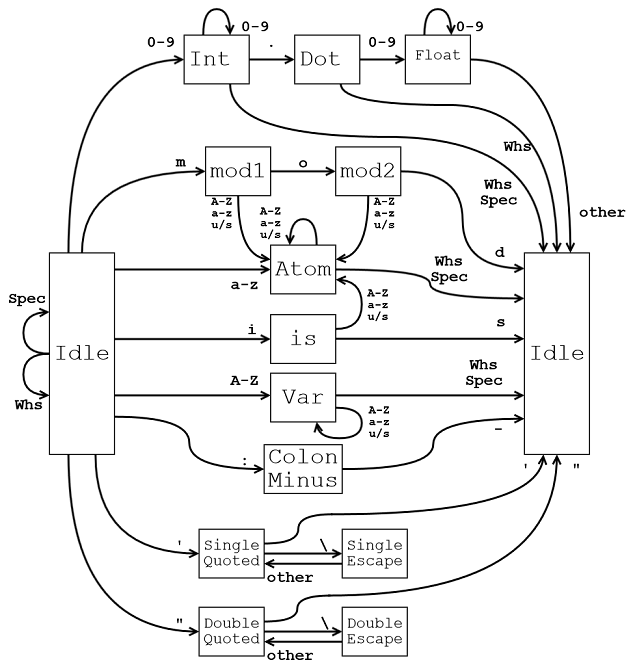
\includegraphics{lex65.png}%[scale=1]{lex.png}
%\end{figure}

\vspace{-10px}
\begin{itemize}
\item \verb|0-9| means any digit.\vspace{-4px}
\item \verb|A-Z| means any uppercase letter.\vspace{-4px}
\item \verb|a-z| means any lowercase letter, excluding those mentioned on another arc.\vspace{-4px}
\item \verb|u/s| means underscore.\vspace{-4px}
\item \verb|Spec| means the set of special characters $\{$\verb/:-.,[]|+*\<>=!`"/$\}$.\vspace{-4px}
\item \verb|Whs| means whitespace: tabs, newlines, spaces.
\end{itemize}

\newpage

For the most part, the state machine moves between an ``idle'' state and the state corresponding to a token being lexed. 
We move to the appropriate state based on the first character lexed. 
Each state has a set of valid characters that contribute to the current token. 
When a character not in this set if encountered, then we transition back to the idle state.
The only case where the first character doesn't tell us the token is for integers and floats. 
We transition to the integer state, and if we encounter a dot character, we transition to parsing a float.
A further inconvenience comes from Prolog's use of the dot character as an end-of-statement marker. 
This means that an integer at the end of a line will have a dot character immediately after it. 
We can still parse unambiguously, because an end-of-statement dot must be followed by whitespace, while a floating-point dot must be followed by a digit. 
It just makes the state machine, and the corresponding code, more complex.

The implementation of the state machine includes a function for each state, with transitions represented by calls to the function of the destination state.

The lexer produces the entire list of tokens before any parsing is done. 
This is less space-efficient than an implementation that lexes the input on-demand to produce the next token in a stream, because the tokens for the entire program must be in memory at once. 
Furthermore, the lexer fails cleanly if there is a syntax error in the source file being tokenised, but doesn't provide any detailed error information, as one might expect from a commercial compiler. 
However, these improvements weren't important to the goals of the project, and thus weren't a priority.

\subsection{Parser}

Once the character stream has been tokenised, the next step in compilation is to build the token stream into an abstract syntax tree. 
Prolog's syntax is representable by a context-free grammar: it is a small language, so the grammar is relatively small. 
Furthermore, it can be written in such a way as to not have left recursion, and can therefore be parsed using the standard recursive descent parsing method. 
The grammar I implemented is as follows:

\newpage

\texttt{
S $\rightarrow$ Lines EOF\\
Lines $\rightarrow$ Line DOT MoreLines\\
MoreLines $\rightarrow$ $\epsilon$ | Lines\\
Line $\rightarrow$ Query | Clause\\
Query $\rightarrow$ COLONMINUS TermList\\
Clause $\rightarrow$ Term Body\\
Body $\rightarrow$ $\epsilon$ | COLONMINUS TermList\\
TermList $\rightarrow$ Term IsTerm MoreTerms\\
IsTerm $\rightarrow$ $\epsilon$ | IS Term IsTerm | EQUALS Term IsTerm\\
MoreTerms $\rightarrow$ $\epsilon$ | COMMA TermList\\
Term $\rightarrow$ ATOM Args | LEFTSQ TermList MoreList | Arith MoreArith\\
.\hspace{20px} | NegArith MoreArith \\
Args $\rightarrow$ $\epsilon$ | LEFTPAREN TermList RIGHTPAREN\\
MoreList $\rightarrow$ RIGHTSQ | PIPE Tail RIGHTSQ\\
Tail $\rightarrow$ VARIABLE | LEFTSQ TermList MoreList\\
Arith $\rightarrow$ ArithTerm MoreArithTerms\\
NegArith $\rightarrow$ NegArithTerm MoreArithTerms\\
MoreArith $\rightarrow$ GREATER ArithTerm MoreArithTerms\\
.\hspace{50px} | LESS ArithTerm MoreArithTerms \\
ArithTerm $\rightarrow$ Factor MoreFactors\\
NegArithTerm $\rightarrow$ MINUS Factor MoreFactors\\
MoreArithTerms $\rightarrow$ $\epsilon$ | PLUS Arith | MINUS Arith\\
Factor $\rightarrow$ INT | FLOAT | LEFTPAREN Arith RIGHTPAREN | VARIABLE | CUT\\
MoreFactors $\rightarrow$ MULT ArithTerm | DIV ArithTerm | MOD ArithTerm
}

The parser is implemented with a function for each non-terminal. 
The function uniquely determines a rule to apply by examining the next token in the stream. 
It then implements that rule by going left-to-right through the symbols on the right-hand-side of that rule, consuming a token from the stream for each terminal in the rule, and calling the relevant function for each non-terminal.

A full treatment of recursive-descent parsing methods is given by Aho et al. \cite{compiler}

The parser for pure Prolog could be implemented by ``pure'' recursive descent. 
However, when arithmetic was added, it was not possible to write grammar rules without left recursion that would give the desired associativity. 
Thus, it was necessary to write non-standard code to implement the grammar correctly: specifically, when parsing arithmetic terms, the earlier terms have to be ``passed along'' as arguments to later recursive calls to build the tree correctly.

As with the lexer, the parser fails cleanly if the token stream cannot be parsed into a valid abstract syntax tree, but it doesn't give detailed error information, because doing so wasn't essential to the goals of the project.

\subsection{Unification}

\subsubsection{The signature}

The unification algorithm takes two arguments. 
The first is a \verb|Unifier| containing all of the variable bindings that have been made so far, which must be respected by the new unification. 
The second is a \verb|Binding|, containing the two terms which are to be unified. 
The output is a pair containing a \verb|bool| and a \verb|Unifier|. 
If the unification is successful, the \verb|bool| will be \verb|true| and the \verb|Unifier| will contain the \verb|Binding|s from the input \verb|Unifier|, the input \verb|Binding|, and any additional \verb|Binding|s required to make the input \verb|Binding| consistent.

\subsubsection{Conditions for success}

In any case where we are unifying terms of different non-variable types, such as an \verb|IntTerm| and a \verb|FloatTerm|, unification fails right away. 

In any case where at least one term to be unified is a variable, we add the input \verb|Binding| to the input \verb|Unifier|. 
If the input \verb|Unifier| was empty, then there can be no inconsistency, so unification succeeds immediately. 
We will see shortly that this is an important base-case for validating \verb|Unifier|s. 
Otherwise, we must call \verb|validateUnifier()| to check that the updated \verb|Unifier| is consistent, as will be described below.

This leaves three cases. 
If both terms are \verb|IntTerm|s, or both terms are \verb|FloatTerm|s, unification succeeds if and only if they are equal, returning the same input \verb|Unifier| because no new \verb|Bindings| were made. 

Finally, if both terms are Prolog \verb|Term|s, then unification succeeds if and only if the \verb|Functor|s are equal, the arities are equal, and the arguments are pairwise unifiable. 
Testing that the arguments are unifiable involves applying the unification function to each pair, with the output \verb|Unifier| from each being the input \verb|Unifier| to the next. 
The final output \verb|Unifier| has already been passed through \verb|validateUnifier()| to test that it is consistent, so it is returned as a success.

\subsubsection{Checking consistency}

%To check that a \verb|Unifier| is consistent, \verb|validateUnifier()| takes the transitive closure of that \verb|Unifier|. 
%That is, if there are two \verb|Binding|s $(A, B)$ and $(B, C)$, then $(A, C)$ is added. 
%It then calls \verb|unify()| on each individual \verb|Binding|, with an empty \verb|Unifier|, to verify that every \verb|Binding| is individually consistent.

When a \verb|Binding| is to be added to a \verb|Unifier|, it is necessary to check that it doesn't introduce any inconsistencies. 
To do this, we check the new \verb|Binding| against all the existing \verb|Binding|s to get a list of transitive \verb|Binding|s. 
Any two \verb|Binding|s $(A,B)$ and $(B,C)$ give a transitive \verb|Binding| $(A,C)$.

These transitive \verb|Binding|s are then checked individually in isolation to see that they are consistent. 
This is done by calling \verb|unify()| with an empty \verb|Unifier| for each \verb|Binding| to be checked. 
If all of these unifications succeed, then the input new \verb|Binding| and all of the transitive \verb|Binding|s are added to the input \verb|Unifier| to give a new candidate \verb|Unifier|.

If the individual unifications did not produce any additional \verb|Binding|s, then the candidate \verb|Unifier| is returned as an answer. 
However, if they did, then each such \verb|Binding| has to be added to the \verb|Unifier| by calling \verb|unify()|, because they themselves may be inconsistent or produce transitive \verb|Binding|s.

To illustrate the consistency check, consider an example. 
Say we have a \verb|Unifier| containing two \verb|Bindings|: \verb|X = foo(A)| and \verb|Y = foo(B)|. 
We call \verb|unify()| to add a new \verb|Binding| \verb|X = Y|. 
The consistency check will add three transitive bindings: \verb|X = foo(B)|, \verb|Y = foo(A)| and \verb|foo(A) = foo(B)|. 
It will then check that each of these transitive bindings is consistent by calling \verb|unify()| with an empty \verb|Unifier|. 
All three will succeed, and we will get a candidate \verb|Unifier| containing all of the bindings mentioned so far.
However, the third unification will generate another new binding \verb|A = B|. 
This new binding has to be added to the candidate \verb|Unifier|, so we call \verb|unify()| with the candidate \verb|Unifier| and this new \verb|Binding| that we wish to add.
Doing so produces no transitive \verb|Binding|s, so the \verb|Binding| is simply added to give a new candidate \verb|Unifier|, which is then returned as the overall answer.

%TODO
%This fact that \verb|unify()| and \verb|validateUnifier()| are mutually recursive should give the reader concern as to whether this algorithm will always terminate. 
%This is a valid question, and a justification will be given later on during evaluation, showing that this will indeed terminate on any valid input.

\subsection{Interpreter}

The input to the interpreter is a \verb|Program| and a list of \verb|Query|s. 
For each query, the aim is to find a \verb|Unifier| that unifies each term in the query with the head of some clause in the program. 
If we visualise a queue of terms that need to be unified with a clause, then the query terms are the initial contents of that queue. 
If the clause with which a term is unified has a body, then the terms in the body also have to be unified with a clause in the program.
The unified term is therefore removed from the queue and the body terms are added to the front of the queue.

%TODO Diagram of queue, unification, expansion

At a given step of execution, there is a term at the front of the queue which must be satisfied, and a list of clauses with which to try to unify it. 
Execution proceeds by taking a clause off the list and attempting the unification. 
There are success and failure continuation functions, which are called based on the outcome of the unification.
The success continuation is the execution of the rest of the terms in the queue. The failure continuation takes another clause from the list, or if the list is empty, backtracks to a previously completed queue item.

%TODO Diagram of continuations

The success continuation takes two arguments: the \verb|Unifier| containing all \verb|Binding|s made so far, and the caller's failure continuation. 
If the next predicate has to backtrack, it can go back to the previous predicate via this failure continuation, and will be at the same position in the clause list as when it left. 
The failure continuation also holds all previous predicates' progress in a similar manner.

%TODO Diagram

It is in this way that we realise the goal described in \S1.4 of retaining information about previous predicates without the WAM's explicit environment stack, by leveraging continuations. 
When a continuation is defined using ML's \verb|let ... in| syntax, ML implicitly creates a closure at run-time containing all relevant state for the continuation function.

\subsection{Compiler}

When running a predicate through the interpreter, it has to search the head of every program clause for a potential unification. 
Depending on the scale of the program, there could be dozens, hundreds or even thousands of clauses to search through, only a tiny number of which are even relevant to the predicate we are trying to evaluate.
This could represent a significant and extremely common run-time overhead. The ambition of the compiler is to eliminate this overhead to achieve a performance gain.

\subsubsection{Overlap With Interpreter}

The compiler uses the same front-end as the interpreter to lex the input file and parse it into an abstract syntax tree. 
It also reuses the unification algorithm and the implementations of built-in predicates (to be discussed in \S3.9). 
However, rather than interpreting the tree, it outputs source ML code to perform the execution.

\subsubsection{Predicate Functions}

Every predicate in the input program is compiled to a function in the output program. 
As a reminder, a predicate is a set of clauses with matching \verb|Functor| symbol and arity. 
The individual clauses are compiled as pattern functions, described below. 
The predicate function builds a chain of failure continuations that call each pattern function in turn, and then calls the first pattern function with this failure continuation and the arguments to the predicate.

\subsubsection{Pattern Functions}

A pattern function first unifies the input arguments with the relevant terms from the head of the clause from which it was created.
If all of these unifications succeed, it builds a chain of success continuations which successively call the predicate functions corresponding to the body terms of the original clause, with the appropriate arguments.

In this way, we have eliminated the linear search through the program clauses, replacing it with direct function calls that branch straight to the useful clauses for the predicate being evaluated.

%TODO other optimisations?

\subsubsection{Query Functions}

Queries are compiled into functions similarly to patterns, with a chain of success continuations to evaluate the query terms in turn. 
Finally, an \verb|execute()| function is added which calls the query functions in turn: separate queries are completely independent, so this is simply a sequence of calls.

\subsection{Variable Substitutions}

In \S1.2.1, I described how when a variable is bound, the term to which it is bound logically replaces all occurrences of that variable. 
Therefore, at some point during or after the execution of a query, the instantiation must be substituted for all occurrences of the variable. 
For example, if we had the bindings \verb|A = a(B)| and \verb|B = b|, and \verb|A| was a query variable, we would want to return \verb|A = a(b)|.

\subsubsection{Substituting at the end}

My initial implementations performed substitution at the very end of a query's evaluation, after all unifications had been completed. 
The algorithm uses two sets of \verb|Binding|s, $A$ and $B$, with $A$ initially containing all of the \verb|Binding|s in the final output \verb|Unifier| and $B$ initially empty.

I say that a \verb|Binding| $x$ is ``expanded'' with respect to a set of \verb|Binding|s $X$ if $x$ contains no variables which are instantiated by a \verb|Binding| in $X$. 
Otherwise, I can ``expand'' $x$ with respect to $X$ by replacing variables in $x$ with their instantiations in $X$.

For each \verb|Binding| $a$ in $A$, I expand $a$ with respect to $B$. 
I then apply $a$ as a substitution to each \verb|Binding| in $B$, and then add $a$ to $B$. 
After each iteration, all bindings in $B$ are expanded with respect to each other. 
When all bindings from $A$ have been added to $B$, then $B$ is the output.

The problem with this approach is that the \verb|Unifier| becomes very large during execution, which slows down verification of new \verb|Binding|s as described in \S3.6.3. 
It is also a large memory overhead, storing the \verb|Binding|s from every successful unification.
To remedy this, I sought out an alternative approach.

\subsubsection{Substituting during execution}

My final implementations perform variable substitutions during execution of a query to eliminate all instances of that variable so that its \verb|Binding|s can be forgotten.
The algorithm performs cleanup every time the end of an executed clause is reached.
All variables local to that clause will be tagged with that clause's scope (recall \S3.2.2).
These variables cannot occur in future predicates' executions, because they are local to the now-complete clause.
So, for any local variables of the completed clause which have been instantiated, we can replace all occurrences of them in the \verb|Unifier| with that instantiation. 
This requires a linear scan through the \verb|Unifier| to find the instantiations of local variables, and for each instantiation found, another linear scan to perform the substitution.
Once this substitution has been done, the instantiation can be removed from the \verb|Unifier|.
This allows us to keep the size of the \verb|Unifier| down as execution proceeds.

An important aspect of this algorithm is that it does not guarantee to clean up all local variables.
A local variable is only cleaned up at the end of its clause, and only if it is instantiated.
If it is not instantiated at that time, then it is never substituted.
In this sense, the implementations safely over-approximate the liveness of local variables.
For this reason, we still have to perform the end-of-execution substitution pass as described in the previous section, which will perform all remaining substitutions.

\subsubsection{Occurs Check}

Substitution gets messy when a variable violates the occurs check, which I described in \S1.2.7. 
When a substitution is to be made, the source binding is checked to see whether the instantiation contains the variable it is instantiating. 
If so, then some fix-up code is executed which performs the substitution correctly. 
This is most clearly explained by example.

Say we have \verb|A = a(A)| and \verb|B = A|. By transitivity, we must also have \verb|B = a(A)|. 
When eliminating \verb|A|, \verb|B = A| is deleted as part of the normal algorithm. 
We then want to substituted \verb|A = a(A)| into \verb|B = a(A)|. 
The former will be detected as an occurs-check case, and the substitution will be changed so that we are substituting \verb|A = B| into \verb|B = a(A)|, which gives \verb|B = a(B)| as we would like.

\subsection{Other Features}

\subsubsection{Scoping}

As mentioned in \S3.2.2, \verb|Variable|s are tagged with a scope number to distinguish them from unrelated variables of the same name, eg: multiple calls to the same clause.
This is simply implemented by having an \verb|int ref| initialised to \verb|2| in the interpreter and compiler to act as a scope counter.
Recall that scope \verb|`1'| is reserved for query variables.
When the interpreter tries to unify the current predicate with a program clause, it first sets the scope of all variables in that clause to the value of the scope counter and increments the counter. 
Similarly, the compiler reads and increments the scope counter's value at the start of a pattern function and uses it for variables in that pattern.

\subsubsection{Cut}

The semantics of Prolog's special cut operator `\verb|!|' were introduced back in \S1.2.6.
It is implemented by introducing an additional ``global fail'' continuation. 
At any given time, this represents the new backtracking point if we were to encounter the cut operator. 
In the interpreter, the fail continuation given at the beginning of a predicate's execution is kept as the global fail continuation for that predicate's execution. 
Similarly in the compiler, the fail continuation supplied as an argument to a predicate function is its global fail continuation, and is passed to each pattern function.
If a cut term is encountered, then it calls the success continuation to evaluate the next term in the clause.
However, rather than passing forward the ``local'' failure continuation that it was given, it passes the global fail continuation, which gives exactly the desired behaviour.

\subsubsection{Built-in Predicates}

The Prolog standard defines a number of built-in predicates which can be used by a program without being defined in the source file, such as \verb|append| for joining two lists or \verb|fail| which always fails. 
While my implementations are by no means exhaustive with respect to supporting these predicates, I included a handful of them to increase the range of sample programs that I could test my implementations on.

These predicates are implemented in an ML source file that both the interpreter and the compiler refer to.
The interpreter tests a predicate to be evaluated against this known list of built-ins before going through the program clauses, and calls the relevant function if it finds a match. 
Similarly, the compiler will output a call to a built-in predicate rather than the usual predicate function if it detects a match.

Some of these predicates can be expressed in Prolog, in which case I wrote them in Prolog and the compiled output was included in the built-in predicates file. Other predicates required non-standard behaviour, such as the `\verb|is|' predicate described below, and I implemented these by hand.

\subsubsection{The `is' Predicate}

As outlined in \S1.2.8, Prolog implementations should not arithmetically evaluate a term unless explicitly instructed to by the presence of the \verb|is| predicate.
This predicate is provided through the built-in predicates system.
When it is called, the second argument is evaluated arithmetically and then unified with the first.
Arithmetic expressions are parsed into a tree of Prolog terms at the parser stage, so evaluation involves doing a post-order treewalk (evaluate both of a node's children before the node) to build up the final result.
When variables are encountered during evaluation, the current \verb|Unifier| is searched for a binding of that variable.
If one is not found, an \verb|UninstantiatedVariable| exception is raised. 

I mentioned when describing the \verb|term| datatype in \S3.2.2 that negative numbers are represented by a positive term with a unary minus parent.
To understand the rationale, consider the expressions \verb|-X + 4|, \verb|Y + 4| and \verb|-9 + 4|. 
Consider unifying any two of these directly, without the \verb|is| predicate. 
If \verb|X| was bound to 9 and \verb|Y| to -9, we would expect success. 
However, how would we represent the fact that \verb|X| was negated?
It would have to have a unary minus parent term.
If the other two expressions simply had \verb|IntTerm|s with negative values, this would require a whole lot of extra logic in the unification algorithm to handle correctly: there wouldn't be a canonical form for terms of this nature.
Similarly, the implementation of \verb|is| would have two different potential tree layouts for negative numbers, and extra care would be needed.
By using the unary minus parent representation everywhere, we get a canonical form.

%TODO Wildcards

\newpage

\section{Evaluation}

% Evaluation and Conclusion: 2400 words

%TODO Speed analysis
% -- Potential future gains

\subsection{Correctness of implementation}

The most important aspect of an implementation of a programming language is correctness. 
A fast implementation is worth nothing if it does not produce the correct result.

To establish the correctness of my implementations, I put together several suites of sample Prolog programs to test it.
By comparing the output of the program when run by my implementations with the output when run with the existing publicly-available SWI-Prolog implementation, I could verify that there was no difference and that my implementations were behaving correctly.

The first suite was a collection of programs that I wrote myself, which were specially targetted at testing specific behaviours of the software.
These included straightforward programs to test basic functionality like simple unifications, as well as more unusual program with uncommon syntax or semantics that would test rare edge cases, like variable names containing numbers and underscores.
Some of the programs contained intentional compile-time or run-time errors, so that I could ensure that these were also handled cleanly and correctly.

I built up this suite of test programs over the course of implementation, expanding it as I added functionality. 
I attempted to cover as broad a range of potential failures as possible. 
When new bugs arose and were fixed, I added additional programs to cover those cases.
Having this suite also allowed me to do regression testing whenever I made significant alterations to the code, such as when I implemented the alternate substitution algorithm as described in \S3.9.

The second collection of programs consisted of real-world programs collected from various online resources.
This collection was put together in the project's evaluation phase to establish further confidence in the correctness of my implementations.

%\subsection{Termination of Unification Algorithm}

%As mentioned in \S3.6, the unification algorithm is implemented by two mutually recursive functions, \verb|unify()| and \verb|validateUnifier()|. The following shows that the algorithm will always terminate.

%[to write]

\subsection{Implementing ML with continuations}

I stated at the beginning that a primary goal of the project was to judge the effectiveness of using continuation-passing style to implement the control flow of Prolog. 
Having completed the implementation, I can say that CPS was a very successful strategy.

The code in the interpreter module of the software is relatively straightforward. 
Execution of any given predicate is passed a success continuation and a failure continuation, and the appropriate continuation is called based on the outcome of the execution, as was described in detail in \S3.7. 
These continuations are easy to define: a series of success continuations are defined by a call to a recursive function that executes each predicate of a clause in turn, and a failure continuation is defined as attempting to execute a predicate using the remaining clauses that haven't been tried yet. 
These calls are already integral to interpreting Prolog code, and applying CPS simply means that we pass these calls around.

The code for the interpreter module is concise, being about 150 lines long. 
It did not take significant development time to write, and no subtle bugs were found in it later on when the programs being executed became more complex. 
It was small, intuitive and maintainable.

\subsection{Implementation problems: the Binding representation}

When it comes to project difficulties which could have been avoided with hindsight, the \verb|Binding| datatype for representing variable bindings is by far the most prominent. 
As was described in detail in earlier sections, variable bindings are handled by keeping a transitive closure of current bindings in a \verb|Unifier| datastructure. 
When a new binding is made by unification, transitive bindings are also added to the \verb|Unifier|.

The major difficulty with this datastructure comes from maintaining it in such a way as to keep it free of clutter. 
Not only is this important for memory efficiency, but in addition, several areas of the code are required to do linear scans of the current \verb|Unifier|, such as the substitution algorithm discussed in \S3.9. 
If we have a lot of extraneous \verb|Binding|s in the \verb|Unifier|, then this will slow down performance considerably.

With this in mind, I imposed the semantics that the unification algorithm would not return a \verb|Unifier| containing any \verb|Binding|s between two non-variables, as these \verb|Binding|s contain no information. 
In practice, correctly enforcing this was conceptually challenging. 
It presented a major hazard for subtle bugs to slip through. 

When I changed my substitution algorithm to perform substitutions during execution, this produced further complications. 
Great care was needed to efficiently eliminate \verb|Binding|s which were no longer useful after substitution: either because they became term-to-term bindings, or because they became duplicates of existing \verb|Binding|s. 
This was another area that needed significant development effort to fully debug to achieve an efficient implementation.

Finally, the occurs check was difficult to handle with this scheme. 
Typical Prolog interpreters don't ever have to perform an occurs-check explicitly, because the internal datastructures they use allow self-reference without trouble.
However, as I described in \S3.9.3, substitutions using my \verb|Binding| representation can give undesirable effects in the presence of self-referencing variables unless an explicit occurs check is performed and appropriate steps are taken.

The \verb|Binding| representation was simply not well-suited to the problem. 
If I were approaching the project again, I would consider a datastructure closer to what the WAM does (\S1.4). 
The WAM focuses on structure-sharing, whereby variables are pointers into a heap of instantiated terms. 
While ML is not necessarily very robust with respect to this low-level view of data, the principle of of having shared structures when variables are bound to each other could be refined into an appropriate concept for a datatype which might be more intuitive and less bug-prone than the \verb|Binding| datastructure I elected to use.

\subsection{Comparison to commercial implementations}

As has already been stressed, completeness of the implementations was not a goal of the project. As such, the final software does not support as rich a feature set as commercial Prolog interpreters like SWI-Prolog and GNU Prolog, lacking more elaborate features like I/O support.

As one might expect, the implementations I wrote in a few months run far more slowly than commercial implementations with years of refinement and teams of developers. I did not collect detailed data to measure this, but an informal comparison with a handful of non-trivial programs indicated a speed difference of several orders of magnitude. A program that took a few seconds in SWI-Prolog took upwards of ten minutes for my implementation.

\subsection{Benefits of compiling to ML}

A more interesting comparison, which I investigated more thoroughly, is the difference in performance between my interpreter and compiler implementations. One of the stated goals of my project was to determine whether there was any gain from pre-compiling Prolog code, compared with simply interpreting it.

It was difficult to collect substantial amounts of data because of the availability of appropriate programs. For a speed analysis, it's necessary to have interesting programs with non-trivial running time. While there is a reasonably plentiful supply of simple Prolog snippets from various tutorials that can be used to test correctness, this was not the case for more elaborate programs. Prolog is a relatively little-used language, so the number of available real programs is correspondingly few. Furthermore, real programs are very likely to use advanced language features, and since my implementations aren't complete, most of these real programs couldn't be run. Nonetheless, I was able to find a few appropriate programs for the comparison.

[ Collect and display data showing the performance gains of the compiler over the interpreter ]

\subsection{Future developments}

While the software implemented for the project was sufficient for its goals, there are aspects which could be improved or expanded if it were to be developed further.

Firstly, as discussed in \S3.4 and \S3.5, neither the lexer nor the parser has detailed error reporting because it wasn't essential to the goals of the project and would take a significant amount of development effort to implement to a satisfactory standard. 
In a commercial compiler, if a syntactic error arose which prevented successful lexing or parsing of the input source file, the compiler would report exactly where in the source file the problem arose, and what the problem was.

Secondly, the current implementations do not support the use of infix operators in prefix notation. 
For example, the valid term \verb|+(1, 2)|, equivalent to \verb|1 + 2|, is not parsed successfully by the current parser grammar. 
The grammar would have to be altered to handle this.

Thirdly, the number of built-in predicates could be expanded significantly. 
The ISO standard for Prolog, ISO/IEC 13211-1, describes a large selection of built-in predicates which are required to be supported by any conforming implementation. 
The current software only provides support for a small subset of these.

%100-line interpreter shows effectiveness of continuations

\newpage

\section{Conclusion}

Both success criteria for the project were met. An interpreter for Prolog programs and a source-to-source compiler from Prolog to ML were written and shown to be correct with a high degree of confidence, through extensive testing. Continuations were found to be a concise and powerful way to express the backtracking behaviour of Prolog. Pre-compilation of a Prolog source program to ML was shown to give significant performance improvements compared to interpreting. The project work proceeded in a steady, structured manner and reached a successful result. 

\begin{thebibliography}{9}

\bibitem{byrd00}
  Jahier, Ducass\'e, Ridoux
  \emph{Specifying Byrd's Box Model with a Continuation Semantics}.
  Electronic Notes in Theoretical Computer Science
  Volume 30, Issue 4,
  April 2000.

\bibitem{wam91}
  Hassan A\"it-Kaci
  \emph{Warren's Abstract Machine: A Tutorial Reconstruction}.
  The MIT Press,
  August 1991.
  
\bibitem{compiler}
  Aho, Sethi, Ullman,
  \emph{Compilers: Principles, Techniques and Tools}.
  Pearson Education,
  1st Edition,
  1986.

\end{thebibliography}

\end{document}
